\documentclass[12pt]{amsbook}
\usepackage[utf8]{inputenc}
\usepackage[
backend=biber,
style=numeric,
maxbibnames=99,
sorting=ynt
]{biblatex}
\usepackage{amsmath,amssymb,amsthm}
\usepackage{tikz}
\usepackage{standalone}
\usepackage{svg}
\usepackage{gensymb}
\usepackage{float}
\usepackage{geometry}
\usepackage{hyperref}
\usepackage{graphicx, animate}
\usepackage{caption, subcaption}
\usepackage{pgffor}
\usepackage{mathtools}
\usepackage{array}
\usepackage{cleveref}
\addbibresource{bibliography.bib}
\usepackage{hyperref,thmtools}
%\usepackage{chngcounter}

\usetikzlibrary{decorations.markings}
\usetikzlibrary{arrows,automata}
\usetikzlibrary{positioning}
\usetikzlibrary{arrows.meta,positioning}

\counterwithin{figure}{chapter}
\counterwithin{section}{chapter}
\counterwithin{table}{chapter}
\counterwithin{subsection}{section}


\linespread{1.5}
\let\cleardoublepage\clearpage
% Override ugly default link
\hypersetup{
  colorlinks   = true, %Colours links instead of ugly boxes
  urlcolor     = blue, %Colour for external hyperlinks
  linkcolor    = blue, %Colour of internal links
  citecolor   = blue    %Colour of citations
}



\begin{document}

\begin{figure}[H]
    \begin{tabular}{llll}
    \begin{subfigure}[c]{0.3\textwidth}
        \centering
        \resizebox{.6\width}{!}{\input{SynthDataDiagrams/methodology1.tex}}
        \label{method net, a}
    \end{subfigure}
    &
    \centering
    \begin{subfigure}[c]{0.3\textwidth}
        \centering
        \resizebox{.6\width}{!}{\documentclass{standalone}
\usepackage{amsmath,amssymb,amsthm}
\usepackage{tikz}
\usetikzlibrary{decorations.markings}
\usetikzlibrary{arrows,automata}
\usetikzlibrary{positioning}
\usetikzlibrary{arrows.meta,positioning}

\begin{document}
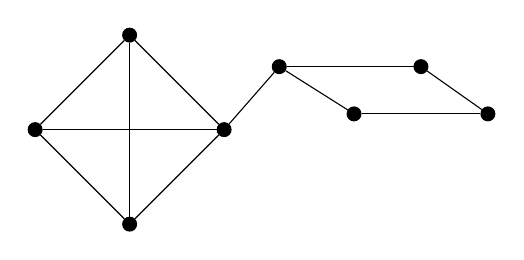
\begin{tikzpicture}[
    mycircle/.style={
        circle,
        draw=black,
        fill=black,
        fill opacity = 1,
        inner sep=0pt,
        minimum size=5pt,
        font=\small},
    nocircle/.style={
        circle,
        draw=black,
        fill=black,
        fill opacity = 1,
        inner sep=0pt,
        minimum size=0.45pt,
        font=\small},
    targetcircle/.style={
        circle,
        draw=red,
        fill=red,
        fill opacity = 1,
        inner sep=0pt,
        minimum size=5pt,
        font=\small},
    myarrow/.style={-},
    dottedarrow/.style={-,dashed},
    thiccarrow/.style={-,line width=0.9pt},
    node distance=1.2cm and 1.5cm
]

\begin{scope}
    \begin{scope}[rotate=90]
        \foreach \x/\y in {0/0,90/1,180/2, 270/3}{ % color in outer layer
        \node[mycircle] (\y) at (canvas polar cs: radius=1.2cm,angle=\x){};
        }
    \end{scope}

    \path[every node/.style={font=\sffamily\small}]
        % (0) edge [color=black] (1)
        (0) edge [color=black] (1)
        (0) edge [color=black] (2)
        (0) edge [color=black] (3)
        (1) edge [color=black] (2)
        (1) edge [color=black] (3)
        (2) edge [color=black] (3);

    \node[mycircle] (a) at (1.9, 0.8) {};
    \node[mycircle] (b) at (2.85, 0.2) {};
    \node[mycircle] (c) at (3.7, 0.8) {};
    \node[mycircle] (d) at (4.55, 0.2) {};

    \path[every node/.style={font=\sffamily\small}]
        (3) edge [color=black] (a)
        (a) edge [color=black] (b)
        (a) edge [color=black] (c)
        (c) edge [color=black] (d)
        (b) edge [color=black] (d);


\end{scope}
\end{tikzpicture}
\end{document}}
        \label{method net, b}
    \end{subfigure}
    &
    $\cdots$
    &
    \centering
    \begin{subfigure}[c]{0.3\textwidth}
        \centering
        \resizebox{.6\width}{!}{\input{SynthDataDiagrams/methodology3.tex}}
        \label{method net, c}
    \end{subfigure}
    
    \end{tabular}
    \caption{Example sequence of networks.}
    \label{method nets}
    
\end{figure}

\begin{figure}[H]
    \centering
        \begin{tabular}{llll}
            $\begin{bmatrix}
                \cdot & 1 & 1 & 1 & \cdot & \cdot & \cdot & \cdot\\
                1 & \cdot & 1 & \cdot & \cdot & \cdot & \cdot & \cdot\\
                1 & 1 & \cdot & 1 & 1 & \cdot & \cdot & \cdot\\
                1 & \cdot & 1 & \cdot & \cdot & \cdot & \cdot & \cdot\\
                \cdot & \cdot & 1 & \cdot & \cdot & 1 & 1 & \cdot\\
                \cdot & \cdot & \cdot & \cdot & 1 & \cdot & \cdot & \cdot\\
                \cdot & \cdot & \cdot & \cdot & 1 & \cdot & \cdot & 1\\
                \cdot & \cdot & \cdot & \cdot & \cdot & \cdot & 1 & \cdot
            \end{bmatrix}$
            &
            $\begin{bmatrix}
                \cdot & 1 & 1 & 1 & \cdot & \cdot & \cdot & \cdot\\
                1 & \cdot & 1 & 1 & \cdot & \cdot & \cdot & \cdot\\
                1 & 1 & \cdot & 1 & 1 & \cdot & \cdot & \cdot\\
                1 & 1 & 1 & \cdot & \cdot & \cdot & \cdot & \cdot\\
                \cdot & \cdot & 1 & \cdot & \cdot & 1 & 1 & \cdot\\
                \cdot & \cdot & \cdot & \cdot & 1 & \cdot & \cdot & 1\\
                \cdot & \cdot & \cdot & \cdot & 1 & \cdot & \cdot & 1\\
                \cdot & \cdot & \cdot & \cdot & \cdot & 1 & 1 & \cdot
            \end{bmatrix}$
            &
            $\cdots$
            &
            $\begin{bmatrix}
                \cdot & 1 & 1 & 1 & \cdot & \cdot & \cdot & \cdot\\
                1 & \cdot & 1 & 1 & \cdot & \cdot & \cdot & \cdot\\
                1 & 1 & \cdot & 1 & \cdot & \cdot & \cdot & \cdot\\
                1 & 1 & 1 & \cdot & \cdot & \cdot & \cdot & \cdot\\
                \cdot & \cdot & \cdot & \cdot & \cdot & 1 & 1 & \cdot\\
                \cdot & \cdot & \cdot & \cdot & 1 & \cdot & 1 & 1\\
                \cdot & \cdot & \cdot & \cdot & 1 & 1 & \cdot & 1\\
                \cdot & \cdot & \cdot & \cdot & \cdot & 1 & 1 & \cdot
            \end{bmatrix}$
            
        \end{tabular}
        \caption{Sequence of sparse adjacency matrices associated with the networks in \cref{method nets}.}
        \label{method adjacency}
    \end{figure}
        


    \begin{figure}[c]{1\textwidth}
        \begin{tabular}{m{0.03\textwidth} m{0.3\textwidth} m{0.26\textwidth} m{0.1\textwidth} l}
        &
            $\begin{bmatrix}
                -0.82  & 0.01\\
                -0.64  & 0.36\\
                -0.95 & -0.76\\
                -0.64 &  0.36\\
                -0.48 &  0.82\\
                -0.17 & -0.40\\
                -0.20 & -0.52\\
                -0.07 &  0.25\\
            \end{bmatrix}$
        
        &
        
            $\begin{bmatrix}
                -0.82  &  0.10\\
                -0.82  &  0.10\\
                -0.90 & -0.58\\
                -0.82  &  0.10\\
                -0.42 &  0.81\\
                -0.13  & -0.64\\
                -0.13  & -0.64\\
                -0.12 &  0.57\\
            \end{bmatrix}$
        
        &
        $\cdots$
        &
        
            $\begin{bmatrix}
                -0.85 &  -0.10\\
                -0.85 &  -0.10\\
                -0.85 &  -0.10\\
                -0.85 &  -0.10\\
                 0.08 &  -0.69\\
                 0.11 &  -0.88\\
                 0.11 &  -0.88\\
                 0.08 &  -0.69\\
            \end{bmatrix}$
        \end{tabular}
        \caption{Sequence of truncated SVDs associated with the networks in \cref{method nets}.}
        \label{method embed}
    \end{figure}
    
    \begin{figure}[c]{1\textwidth}
        \begin{tabular}{llll}
        \begin{subfigure}[c]{0.31\textwidth}
            \centering
            \begin{subfigure}[p]{1\textwidth}
                \includegraphics[width=\linewidth]{../Code/Plots/examples/plot 1.png}
                
            \end{subfigure}

        \end{subfigure}
        &
        \centering
        \begin{subfigure}[c]{0.31\textwidth}
            \centering
            \begin{subfigure}[p]{1\textwidth}
                \includegraphics[width=\linewidth]{../Code/Plots/examples/plot 2.png}
                
            \end{subfigure}
        \end{subfigure}
        &
        $\cdots$
        &
        \centering
        \begin{subfigure}[c]{0.31\textwidth}
            \centering
            \begin{subfigure}[p]{1\textwidth}
                \includegraphics[width=\linewidth]{../Code/Plots/examples/plot 3.png}
               
            \end{subfigure}
        \end{subfigure}
        
        \end{tabular}
        \caption{Sequence of embedded points associated with the networks in \cref{method nets}.}
        \label{method plots}
        
    \end{figure}



\end{document}